% !Mode:: "TeX:UTF-8"
\chapter{H.265 帧内无损编码及优化算法硬件实现}
\label{cha:c4}
在视频实时编码的场景中,使用专用集成电路 (Application Specific Integrated Circuit, ASIC) 实现可做到功耗与性能的良好平衡,是业界的主流做法。本章介绍 H.265 帧内无损编码的 ASIC 实现,并给出行为级仿真结果。

\section{硬件系统框架}
如图 \ref{fig:HardwareArch} 所示,H.265 帧内无损编码器包含的主要模块有:帧内预测模块(分为 2 个阶段进行)、熵编码模块、环路后处理模块、变换量化模块(无损编码时跳过处理)以及与外部存储器交互的 Fetch 与像素 Buffer 模块,同时存在大量用于待编码系数的中间缓存模块,不一一列出。
\begin{figure}[hbt]
    \centering
    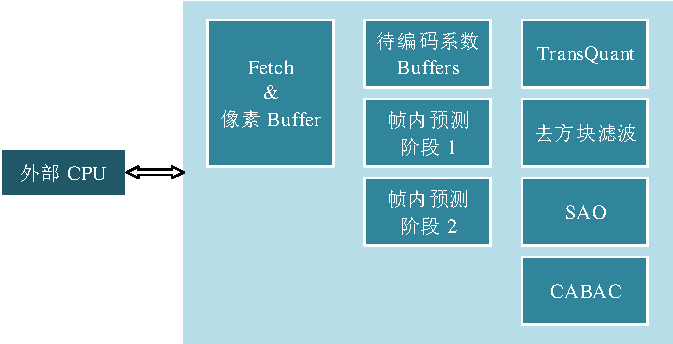
\includegraphics{HardwareArch.pdf}
    \caption{H.265 编码器硬件系统框架}
    \label{fig:HardwareArch}
\end{figure}

图中的外部 CPU 并非系统框架内的模块,系统框架预留了与外部控制器的交互接口,用于进行诸如感兴趣区域 (Range of Interest, ROI)、码率控制、时延控制等外部控制操作。

\section{关键模块的硬件实现}
\begin{itemize}
    
\end{itemize}

\section{行为级仿真与测试}
% 软件编码结果文件比对
% TSMC 65 nm 400MHz 71+138+764+198+125+103K Logic gate count

\section{本章小结}